\documentclass{article}

\usepackage{pgf,tikz,pgfplots}
\pgfplotsset{compat=1.15}
\usepackage{mathrsfs}
\usetikzlibrary{arrows}
\usepackage{amsmath,amssymb}
\usepackage{fullpage}
\usepackage{enumerate}
\usepackage{hyperref}
\usepackage{graphicx}
\graphicspath{{../logos/}}


\begin{document}

\setlength{\tabcolsep}{6pt}
\begin{center} \begin{tabular}{cccc}
	
\includegraphics[height=56pt]{SAMF_logo.jpg} &
	
\includegraphics[height=56pt]{SAICA_logo.jpg} &
	
\includegraphics[height=56pt]{OM_Logo_Stacked_Vignette_on_White_RGB.jpg} &
	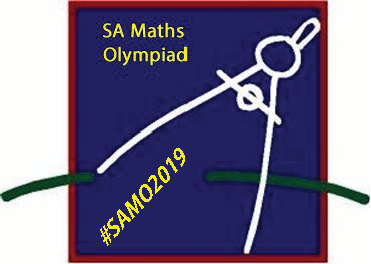
\includegraphics[height=56pt]{SAMO2019.png}
\end{tabular} \end{center}


\bigskip


\begin{center}
	\textbf{\Large Senior February Monthly Problem Set Solutions}
\end{center}

\begin{enumerate}

\medskip
\item % Malwande
{\itshape Let $ABC$ be a triangle with orthocentre $H$, such that $AB<BC$ and $\angle BAC < 90^\circ$. Let the circle $\Gamma$ centred at $B$ and passing through $A$ intersect $AC$ again at $D$. The circumcircle of $\triangle BCD$ intersects $\Gamma$ again at $E$. $ED$ and $BH$ intersect at $F$. Prove that $BD$ is tangent to the circumcircle of $\triangle DHF$.
}
\medskip
\definecolor{wrwrwr}{rgb}{0.3803921568627451,0.3803921568627451,0.3803921568627451}
\definecolor{rvwvcq}{rgb}{0.08235294117647059,0.396078431372549,0.7529411764705882}
\begin{tikzpicture}[line cap=round,line join=round,>=triangle 45,x=1cm,y=1cm]
\clip(-8,-5) rectangle (8,6);
\draw [line width=0.5pt,color=wrwrwr] (-1.38,3.06)-- (-2.4,0);
\draw [line width=0.5pt,color=wrwrwr] (2,0)-- (-1.38,3.06);
\draw [line width=0.5pt,color=wrwrwr] (-2.4,0)-- (2,0);
\draw [line width=0.5pt,color=wrwrwr] (-2.4,0) circle (3.2255232133717473cm);
\draw [line width=0.5pt,color=wrwrwr] (-2.4,0)-- (0.5438098903213396,1.3183259572830477);
\draw [line width=0.5pt,color=wrwrwr] (-1.38,-9.12) -- (-1.38,8.172);
\draw [line width=0.5pt,color=wrwrwr,domain=-11.072:14.03] plot(\x,{(-8.112-3.38*\x)/-3.06});
\draw [line width=0.5pt,color=wrwrwr] (-0.2,-0.9666666666666669) circle (2.403007375029141cm);
\draw [line width=0.5pt,color=wrwrwr,domain=-11.072:14.03] plot(\x,{(--0.15523155666730615--4.378325957283048*\x)/1.9238098903213392});
\draw [line width=0.5pt,color=wrwrwr,domain=-11.072:14.03] plot(\x,{(--2.431982297479315--0.19165929061638076*\x)/1.9238098903213396});
\begin{scriptsize}
\draw [fill=wrwrwr] (-1.38,3.06) circle (2.5pt);
\draw[color=wrwrwr] (-1.194,3.541) node {$A$};
\draw [fill=wrwrwr] (-2.4,0) circle (2.5pt);
\draw[color=wrwrwr] (-2.6,0.37) node {$B$};
\draw [fill=wrwrwr] (2,0) circle (2.5pt);
\draw[color=wrwrwr] (2.172,0.453) node {$C$};
\draw [fill=wrwrwr] (0.5438098903213396,1.3183259572830477) circle (2pt);
\draw[color=wrwrwr] (0.72,1.737) node {$D$};
\draw [fill=wrwrwr] (-1.38,1.126666666666667) circle (2pt);
\draw[color=wrwrwr] (-1.194,1.561) node {$H$};
\draw [fill=wrwrwr] (-1.38,-3.06) circle (2pt);
\draw[color=wrwrwr] (-1.194,-2.641) node {$E$};
\draw [fill=wrwrwr] (2.1944160092360985,5.074877814123534) circle (2pt);
\draw[color=wrwrwr] (2.5,5.2) node {$F$};
\end{scriptsize}
\end{tikzpicture}
We will first show that $H$ lies on the circumcircle of $\triangle BCD$ 
\\ Since $AB = BD$ and $BH \perp AD$, then $AH$ bisects $AD$, then $AH = HD \implies \angle HAD = \angle HDA$. Now $\angle HBC = 90^{\circ} - \angle ACB = \angle HAC$ and so $\angle HBC = \angle HDA$ and so $BHDC$ is cyclic. 
\\ Next we show that $A$, $H$ and $E$ are collinear
\\It is equivalent to to show that $\angle HED = \angle AED$. 
\\ $\angle HED = \angle HBD$ since $BHDC$ is cyclic. 
\\ Also, $\angle AED = \frac{\angle ABD}{2} = \angle HBD$ and so $A$, $H$ and $E$ are collinear. 
\\ Since $\angle ABF = \angle AEF$, then $ABEF$ is cyclic and so $\angle HFD = \angle BAH = 90^{\circ} - \angle ABC = \angle HCB = \angle HDB \implies BD$ is tangent to the circumcircle of $ \triangle DHF$



\medskip
\item % IMO Long List 1992 Q65, A
{\itshape For any 4 points in $\mathbb{R}^3$, does there exist a plane such that the orthogonal projections of the points on the plane make up the vertices of a parallelogram?

}
Let $A,B,C,D$ be vectors from the origin to the $4$ respective points.
And let $p_U(v)$ denote the projection of $v$ onto $U$ for a plane $U$ that goes through the origin. It is well known that $p_U(v) + p_U(w) = p_U(v + w)$

We want to find a plane, $U$, such that the projections of $A$, $B$, $C$ and $D$ are a parallelogram. This is equivalent to
$p_U(A) - p_U(B) = p_U(D) - p_U(C)$

But by additivity of $p_U$ the above is equivalent to
$p_U(A - B + C - D) = 0$

Which means all we need is a plane $U$ through the origin that is perpendicular to $A - B + C - D$, which clearly exists.

In the case where $A - B + C - D = 0$, any plane $U$ would result in a parallelogram.

\medskip
\item % IMO Long List 1992 Q75, N
{\itshape Find all positive integers $n$ that can be written in the form:
$$n = \left\lfloor m + \sqrt{m} + \frac{1}{2} \right\rfloor$$
where $m$ is also a positive integer.}

All positive integers except those that are perfect squares can be written in this form. 
\\ Let $k^{2} \leq m < (k+1)^{2}$ and let $m = k^{2} + x$ where $x \in \{0,1,...,2k\}$
\\ Now consider when $x=\{0,1,2,...,k\}$, then $m \leq k^{2} + k \implies m < k^{2} + k + \frac{1}{4} = (k+\frac{1}{2})^{2}$ and so $\sqrt{m} < k + \frac{1}{2}$
Then $n = \left\lfloor m + \sqrt{m} + \frac{1}{2} \right\rfloor = m + \left\lfloor  \sqrt{m} + \frac{1}{2} \right\rfloor = m + k$. Taking all possible values for $m$ gives that the numbers $n$ that can be formed are $\{k^{2}+k, k^{2}+k+1,..., k^{2}+2k\}$ $\forall k \in \mathbb{N}$
\\ Then consider when $x=\{k+1,k+2,,...,2k\}$, then $m > k^{2} + k \implies m > k^{2} + k + \frac{1}{4} = (k+\frac{1}{2})^{2}$ and so $\sqrt{m} > k + \frac{1}{2}$
Then $n = \left\lfloor m + \sqrt{m} + \frac{1}{2} \right\rfloor = m + \left\lfloor  \sqrt{m} + \frac{1}{2} \right\rfloor = m + k + 1$. Taking possible values for $m$ gives that the numbers $n$ that can be formed are $\{k^{2}+2k+2, k^{2}+2k+3,..., k^{2}+3k+1\}$ $\forall k \in \mathbb{N}$ Letting $k \to k-1$ here generates the set $\{k^{2}, k^{2}+1,...,k^{2}+k\}$. 
\\ In total we can produce numbers only in the form $\{k^{2}+1, k^{2}+2,..., k^{2}+2k\}$ $\forall k \in \mathbb{N}$ which is clearly all the positive integers except the perfect squares. 



\medskip
\item % A Russian Olympiad 1975, C
{\itshape An $8 \times 8$ chessboard is divided into several regions by 13 straight lines. Can the lines be placed in such a way that each region contains at most 1 centre of the original 64 squares?}

Construct the centers of all $28$ outer edge squares, and connect the adjacent centers, resulting in the outline of a square with $28$ segments, $7$ per side. If, after the lines have been placed, there exists one of these segments which have not been crossed, it implies that these $2$ centers lie on the same region. 
Note that a line can pass through at most $2$ of these segments, meaning that there is at least $2$ segments which are uncrossed, resulting in two centers being on the same region.


\medskip
\item % Adapted from Sharygin 2005, G11 P1, G
{\itshape Let the midpoints of the sides $BC$, $CA$, $AB$ of an equilateral triangle $ABC$ be $D$, $E$, and $F$ respectively. Let $j$, $k$, and $\ell$ be lines passing through $D$, $E$, and $F$ respectively such that $j \parallel k \parallel \ell$. Define points $P$, $Q$, and $R$ by $P = j\cap EF$, $Q = k \cap FD$, and $R = \ell \cap DE$. Prove that the points $X$, $Y$, and $Z$ defined by $X = BC \cap QR$, $Y = CA \cap RP$, and $Z = AB \cap PQ$ are  collinear.}



\medskip
\item % Mongolia 2008 TST Day 3 Q3
{\itshape Show that there are only finitely many solutions $(x, y) \in \mathbb{N}^2$ to the equation
$$\sum_{i = 1}^{m} (x + i)^n = \sum_{i = 1}^{m} (y + i)^{2n}$$
where $m, n \in \mathbb{N} \setminus \{1\}$ are given constants.}

By the Power-Mean Inequality, we have:
$$(\frac{(x + i)^n + (x + m + 1 - i)^n}{2})^{\frac{1}{n}} > x + \frac{m + 1}{2}$$
$$\implies \frac{(x + i)^n + (x + m + 1 - i)^n}{2} > (x + \frac{m + 1}{2})^n$$
$$\implies \sum_{i = 1}^{n} (x + i)^n > m(x + \frac{m + 1}{2})^n$$

Expanding the LHS gives:
$$\sum_{i = 1}^{m} (x + i)^n = mx^n + \frac{mn(m + 1)}{2}x^{n - 1} + O_1(x^{n - 2})$$

Similarly:

$$m(x + \frac{m + 2}{2})^n = mx^n + \frac{mn(m + 2)}{2}x^{n - 1} + O_2(x^{n - 2})$$

Since the coefficients of the second term will dominate the expression after subtracting the two, we have:

$$m(x + \frac{m + 2}{2})^n > \sum_{i = 1}^{m} (x + i)^n > m(x + \frac{m + 1}{2})^n ~\forall x > T$$

where $T$ is some sufficiently large real number. Following a similar process and replacing $n$ by $2n$ and $x$ by $y$, we get:

$$m(y + \frac{m + 2}{2})^{2n} > \sum_{i = 1}^{m} (y + i)^{2n} > m(y + \frac{m + 1}{2})^{2n} ~\forall y > K$$

where $K$ is some sufficiently large real number. Adding $1$ to $y$ yields:

$$m(y + \frac{m + 2}{2} + 1)^{2n} > \sum_{i = 1}^{m} (y + i + 1)^{2n} > m(y + \frac{m + 1}{2} + 1)^{2n} ~\forall y > K$$

Since $m$ is fixed, we can choose $y > K$ such that: 
$$y^2 + (m + 2)y + (\frac{m + 2}{2})^2 - \frac{m + 1}{2} > T$$

\medskip
\item % Spain, Round 2, 1992
{\itshape In the land of Graphopia there are $n$ towns. Between some pairs of towns there are direct roads. The residents of these towns want to have mathematics tournaments. They've decided that in order to have a mathematics tournament they need to have $a$ participating towns. Further they decide that in order to have a tournament the connections between the towns involved must be symmetrical. That is either every pair of towns in a tournament are directly linked by a road or no pair is. 

As mathematics competitions are rightly adored by every member of Graphopia every grouping of $a$ towns that can hold a tournament holds one once a year (some towns may be in multiple groupings). However in some years new roads are built and old ones lost to the elements. If a group of $a$ towns find themselves able to put on a tournament they immediately do. If a tournament finds itself unallowable due to road connections, that tournament is regretfully discontinued. Prove that it is possible that one year poor Graphopia finds itself having less than $\binom{n}{a} $$2^{1-\binom{a}{2}}$ tournaments.
}


Let the towns be nodes of a connected graph. If there is a road between two towns, let the edge be coloured red, and blue if not.
Consider the sample-space, $\Omega$, of all possible colourings of the graph and note that each edge has equal frequency and therefor equal probability of being either red or blue for a randomly selected colouring.

Therefor a collection of $a$ towns has probability $2^{1-{{a}\choose{2}}}$ of being mono-coloured.

Let the number of competitions be denoted by ${X}$.

Note that the number of collections of $a$ towns is ${n}\choose{a}$

Now, by Linearity of Expectation: 

$\mathbb{E}({X}) = {{n}\choose{a}}\times2^{1-{{a}\choose{2}}}$

Ignoring the trivial case of $a=2$, since $X$ is discrete and there exists a colouring where $X>\mathbb{E}({X})$, namely the graph where all edges are blue, there must exist a colouring where $X$ is less than $\mathbb{E}({X})$.

\medskip
\item % Serbian Mathematical Olympiad 2007
{\itshape For positive real numbers $a$, $b$, and $c$ with $a+b+c=1$ prove that:
\begin{align*}
 	\frac{a^{n+2}}{a^{n+1} + b^n + c^n} + \frac{b^{n+2}}{a^n + b^{n+1} + c^n} + \frac{c^{n+2}}{a^n + b^n + c^{n+1}} \ge \frac{1}{7}
\end{align*}

where $n \in \mathbb{N}$. Where does equality occur?}


\end{enumerate}

\end{document}
